
    \begin{abstract_online}{Study of Water Extraction by Phosphate Ligands by Experiments and Molecular Simulations}{%
        D. U. Bapat, \underline{V. H. Dalvi}}{%
        \IStag}{%
        Department of Chemical Engineering, Institute of Chemical Technology, Mumbai}
    Molecular level insights into structure-property relationships are essential in order to design high performance materials and chemicals. Although the first and preferred line of attack for such problems is direct experimental measurements, often puzzling aspects of macroscopic behavior of systems are hard, if not impossible, to probe experimentally at current technological levels. In such cases, molecular simulations play an invaluable role in providing microscopic insights into molecular level interactions and can thus guide experiments towards discovery or development of new materials.  This talk will illustrate this point using the example of the partitioning of water into an organic phase containing phosphate ligands. Such systems are backbone of processes for reprocessing spent nuclear fuels since ligands are available that can selectively extract certain actinides from the aqueous to the organic phase.  The conventional model for such partitioning is a reverse micelle of water solvated by the phosphate ligands[1]. The experimental behavior of water partitioning into a dodecane phase containing a mixture of tri-n-butylphosphate (TBP) and di-2-ethylhexylphosphoric acid (D2EPHA) ligands is counterintuitive according to this model since the D2EPHA ligand system containing both hydrogen bond donor and acceptor groups is a weaker extractant of water than a system with TBP ligands which only possess an h-bond acceptor group. Molecular simulations showed that, instead of being present in the core of a reverse micelle, water actually acts as a bridge between phosphate ligand molecules thus forming a range of supramolecular clusters: with as much as $80 \%$ of water’s hydrogen bonds being formed with the extractant molecules rather than other water molecules[2]. \begin{center}  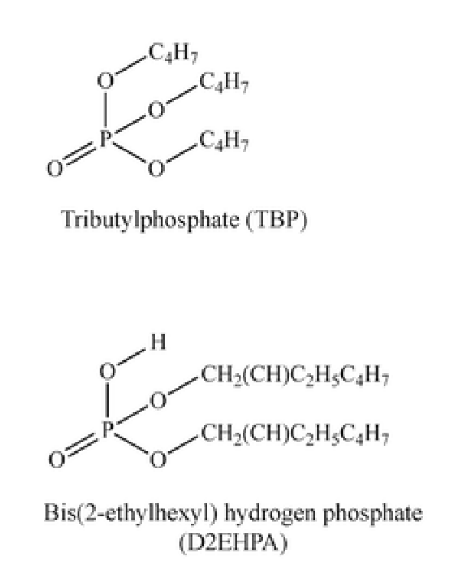
\includegraphics[scale=0.3]{abstracts/txt/figures/vishwa1.png}  \caption{\textbf{Figure 1:} Chemical Structure of the Phosphate Ligands}  \end{center}  \begin{center}  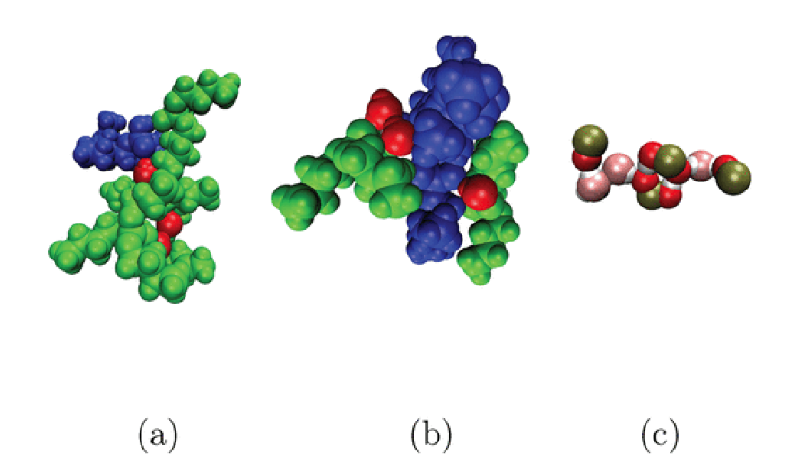
\includegraphics[width=\linewidth]{abstracts/txt/figures/vishwa2.png}  \caption{\textbf{Figure 2:} Representative figures of clusters formed are shown in parts a and b. Extractants are depicted as VDW spheres. Water, D2EHPA, and TBP molecules are colored in red, blue, and green, respectively. In structure c, the cluster depicted in part b is shown without alkyl chain carbons and hydrogens. The cluster is rotated favorably to show the hydrogen bonding centers in the cluster. Red spheres represent the oxygens on the extractants, dark green sphere represents the phosphorus atom, and white spheres represent the hydroxyl hydrogens. Pink spheres represent water molecule oxygen (virtual site and oxygen atom).}  \end{center}  
    
        \textbf{References} \newline{}[1] Osseo-Asare Advances in Colloid and Interface Science (1991) Vol.37 Page 123-173\newline{}[2] Bapat and Dalvi, J. Phys. Chem. B (2019) Vol.123(7) Page 1618-1635 
    \end{abstract_online}
    